 \documentclass[a4paper,10pt]{article}
\input{/Users/WannaGetHigh/workspace/latex/macros.tex}

\title{Rapport TP3 : SMA - Billes / Shelling / proies-pr\'edateurs / Cinq ou plus}
\author{Fran\c{c}ois \bsc{Lepan} - Alexis \bsc{Linke}}

\begin{document}
\maketitle

\section{Choix}

\subsection{Billes}
Nous sommes partis sur un syst\`eme de d\'eplacement sur une grille case par case. Deux agents ne peuvent  se retrouver sur une m\^eme case.

Nous avons fait ce choix car le syst\`eme de collision ainsi que la repr\'esentation sur un \verb&JPanel& est plus facile \`a g\'erer qu'un syst\`eme de d\'eplacement libre.

Les couleurs des Billes sont fix\'es lors de leurs cr\'eation. \\

\subsection{Schelling}

Pour repr\'esenter le mod\`ele de Schelling nous avons choisi une population divis\'ee en deux type : la population bleue et la population jaune, d'\'egale importance. Chaque membre peut regarder dans le voisinage de Moore pour estimer son niveau de satisfaction et s'il n'est pas satisfait il se t\'el\'eporte al\'eatoirement dans l'environnement. Un fichier \emph{Schelling.txt} est cr\'e\'e lors de l'ex\'ecution du code donnant le taux de satisfaction sur la dur\'ee de la simulation. \\

\subsection{Proies - Pr\'edateur}

Pour le mod\`ele proies - pr\'edateur nous avons avons choisis de cr\'eer deux sous classe de Agent l'un pour les proies et l'autre pour les pr\'edateurs. Les positions ainsi que les directions sont d\'efini al\'eatoirement lors de la cr\'eation de ces deux Agents. L'environnement de d\'eplacement est torique.
Deux fichier sont cr\'eer lors de la simulation : \\

\begin{itemize}
\item \emph{ages\_prey\_pred.txt} : contenant les ages de tous les agents \`a chaque tour de simulation.
\item \emph{population\_prey\_pred.txt} : contenant le nombre de proie et de pr\'edateur \`a chaque tour de simulation.
\end{itemize}

\newpage

\subsection{5 ou plus}

Pour le jeu du cinq ou plus nous avons cr\'e\'e quatre classes : \\ 

\begin{itemize}
\item \emph{Plan}: Qui est l'environnement ou se d\'eplace les Agents,
\item \emph{Player}: qui est l'agent qui demande \`a l'utilisateur d'entr\'e des coordonn\'ees,
\item \emph{Token}: qui est l'agent qui regarde si il forme une ligne ou non avec d'autre de ses cong\'en\`ere
\item \emph{MAS\_FiveOrMore}: qui est Le System Multi-agent pour cette simulation.
\end{itemize}
~\\

Voici le d\'eroulement pour ce jeu tout par tour: \\

\begin{itemize}
\item Trois jetons sont cr\'e\'es et positionn\'es sur l'environnement,
\item les jetons regardent un \`a un si ils forment une ligne de cinq ou plus,
\item on v\'erifie si le plateau de jeu est plein,
\item on retire les jetons qui forment une ligne de cinq ou plus du m\^eme type,
\item on met \`a jour la vue de l'environnement
\item et enfin le joueur choisi de faire un d\'eplacement.
\end{itemize} ~\\

Pour la v\'erification de pr\'esence d'une ligne de cinq ou plus, chaque jeton regarde dans quatre directions sur huit (en haut \`a droite, \`a droite, en bas a droite et en bas). Cela suffit car il y aura au moins un jeton sur cinq qui trouvera la ligne \`a enlever. \\

Pour la recherche du chemin le plus cour (\emph{cf.}~Fig.~\ref{recherche_chemin_plus_cour}): \\
\begin{Verbatim}[commandchars=\\\{\}]
On initialise un tableau de Integer de la meme taille que l'environnement avec :
	- 0 pour l'arrive
	 integer.MAX_VALUE pour les agents d\'ej\`a pr\'esent.

Pour (tous les indices des voisins trouv\'e) 
	Pour les case autour de l'agent courant
		Si la case est vide
			on met sa valeur +1
			on rajoute cet agent dans la liste des voisins trouv\'e
		Sinon si l'agent pr\'esent est le depart
			on sort de la boucle -> il y a un chemin
		fin si
	fin pour
fin pour

Si on est sortie de la boucle avant la fin -> il y a un chemin
sinon on redemande un chemin \`a l'utilisateur
\end{Verbatim}

\begin{figure}[ht]
\begin{center}
	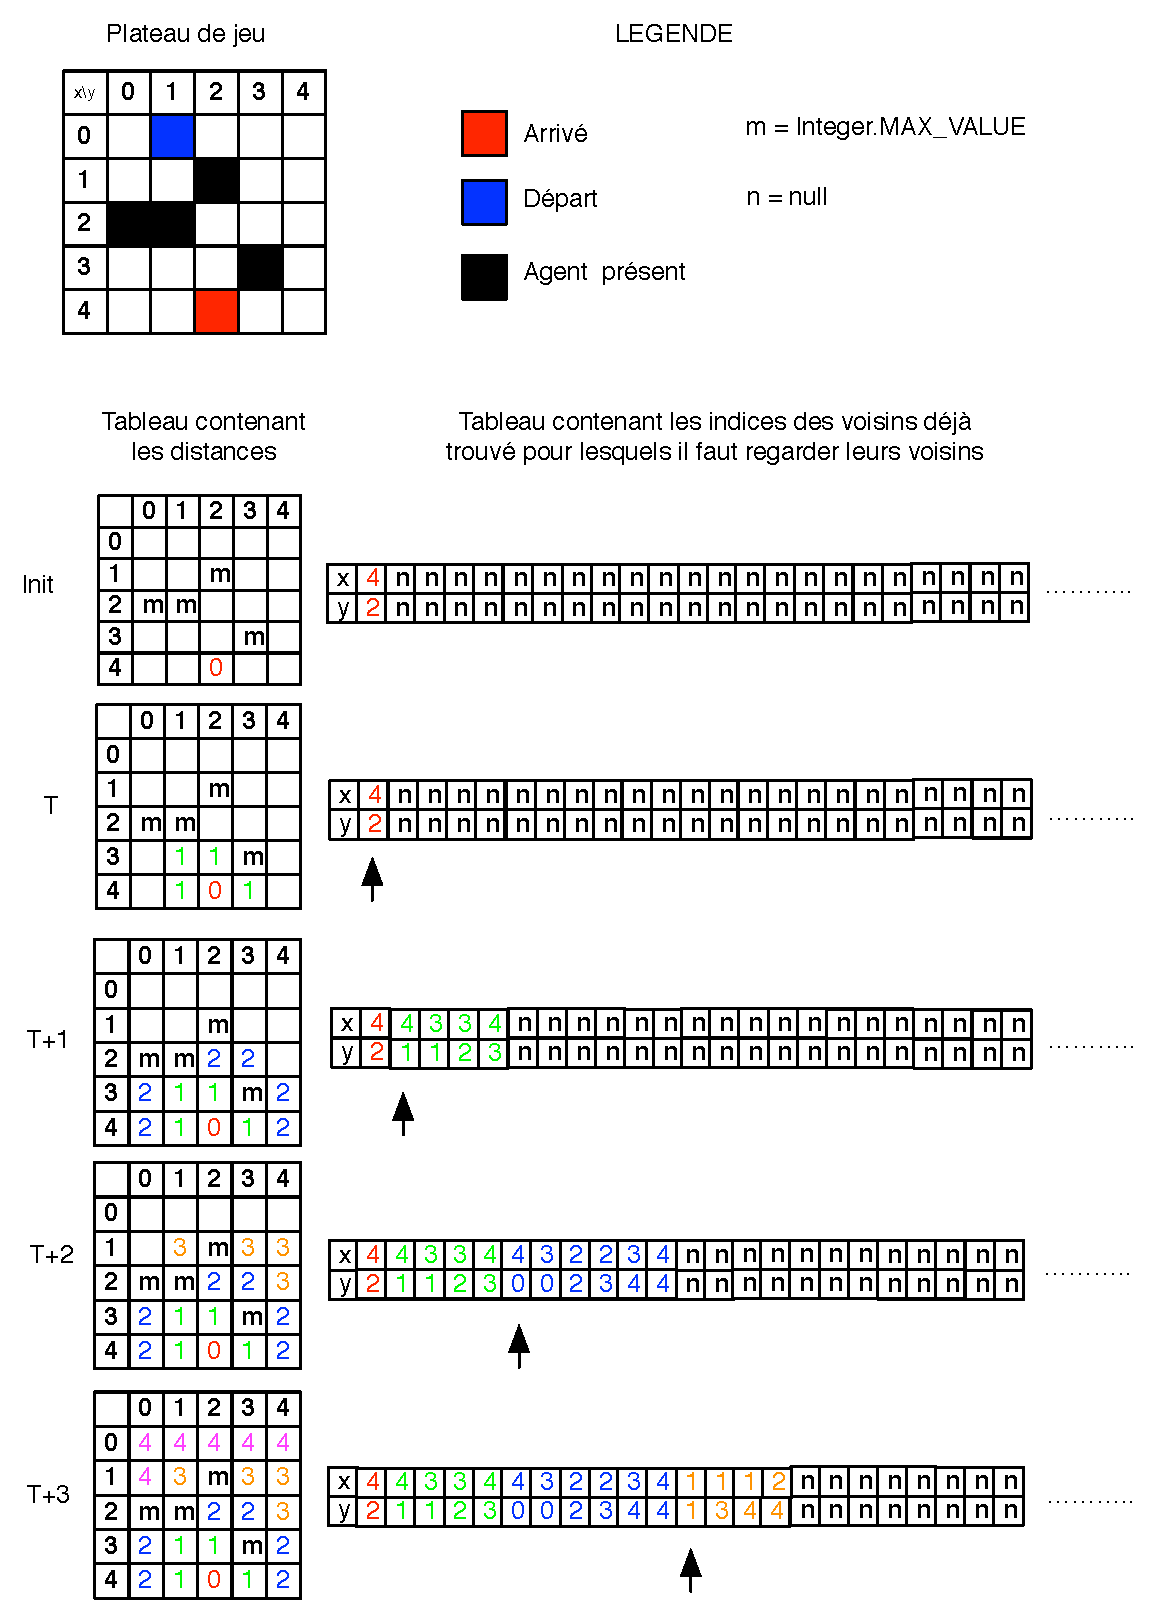
\includegraphics[width=14cm]{images/recherche_chemin_plus_cour}
\end{center}
	\caption{Recherche du chemin le plus cour}
	\label{recherche_chemin_plus_cour}
\end{figure}

\section{UML}

~Fig.~\ref{uml} (Il est aussi disponible en .png dans l'archive)

\begin{figure}[ht]
\begin{center}
	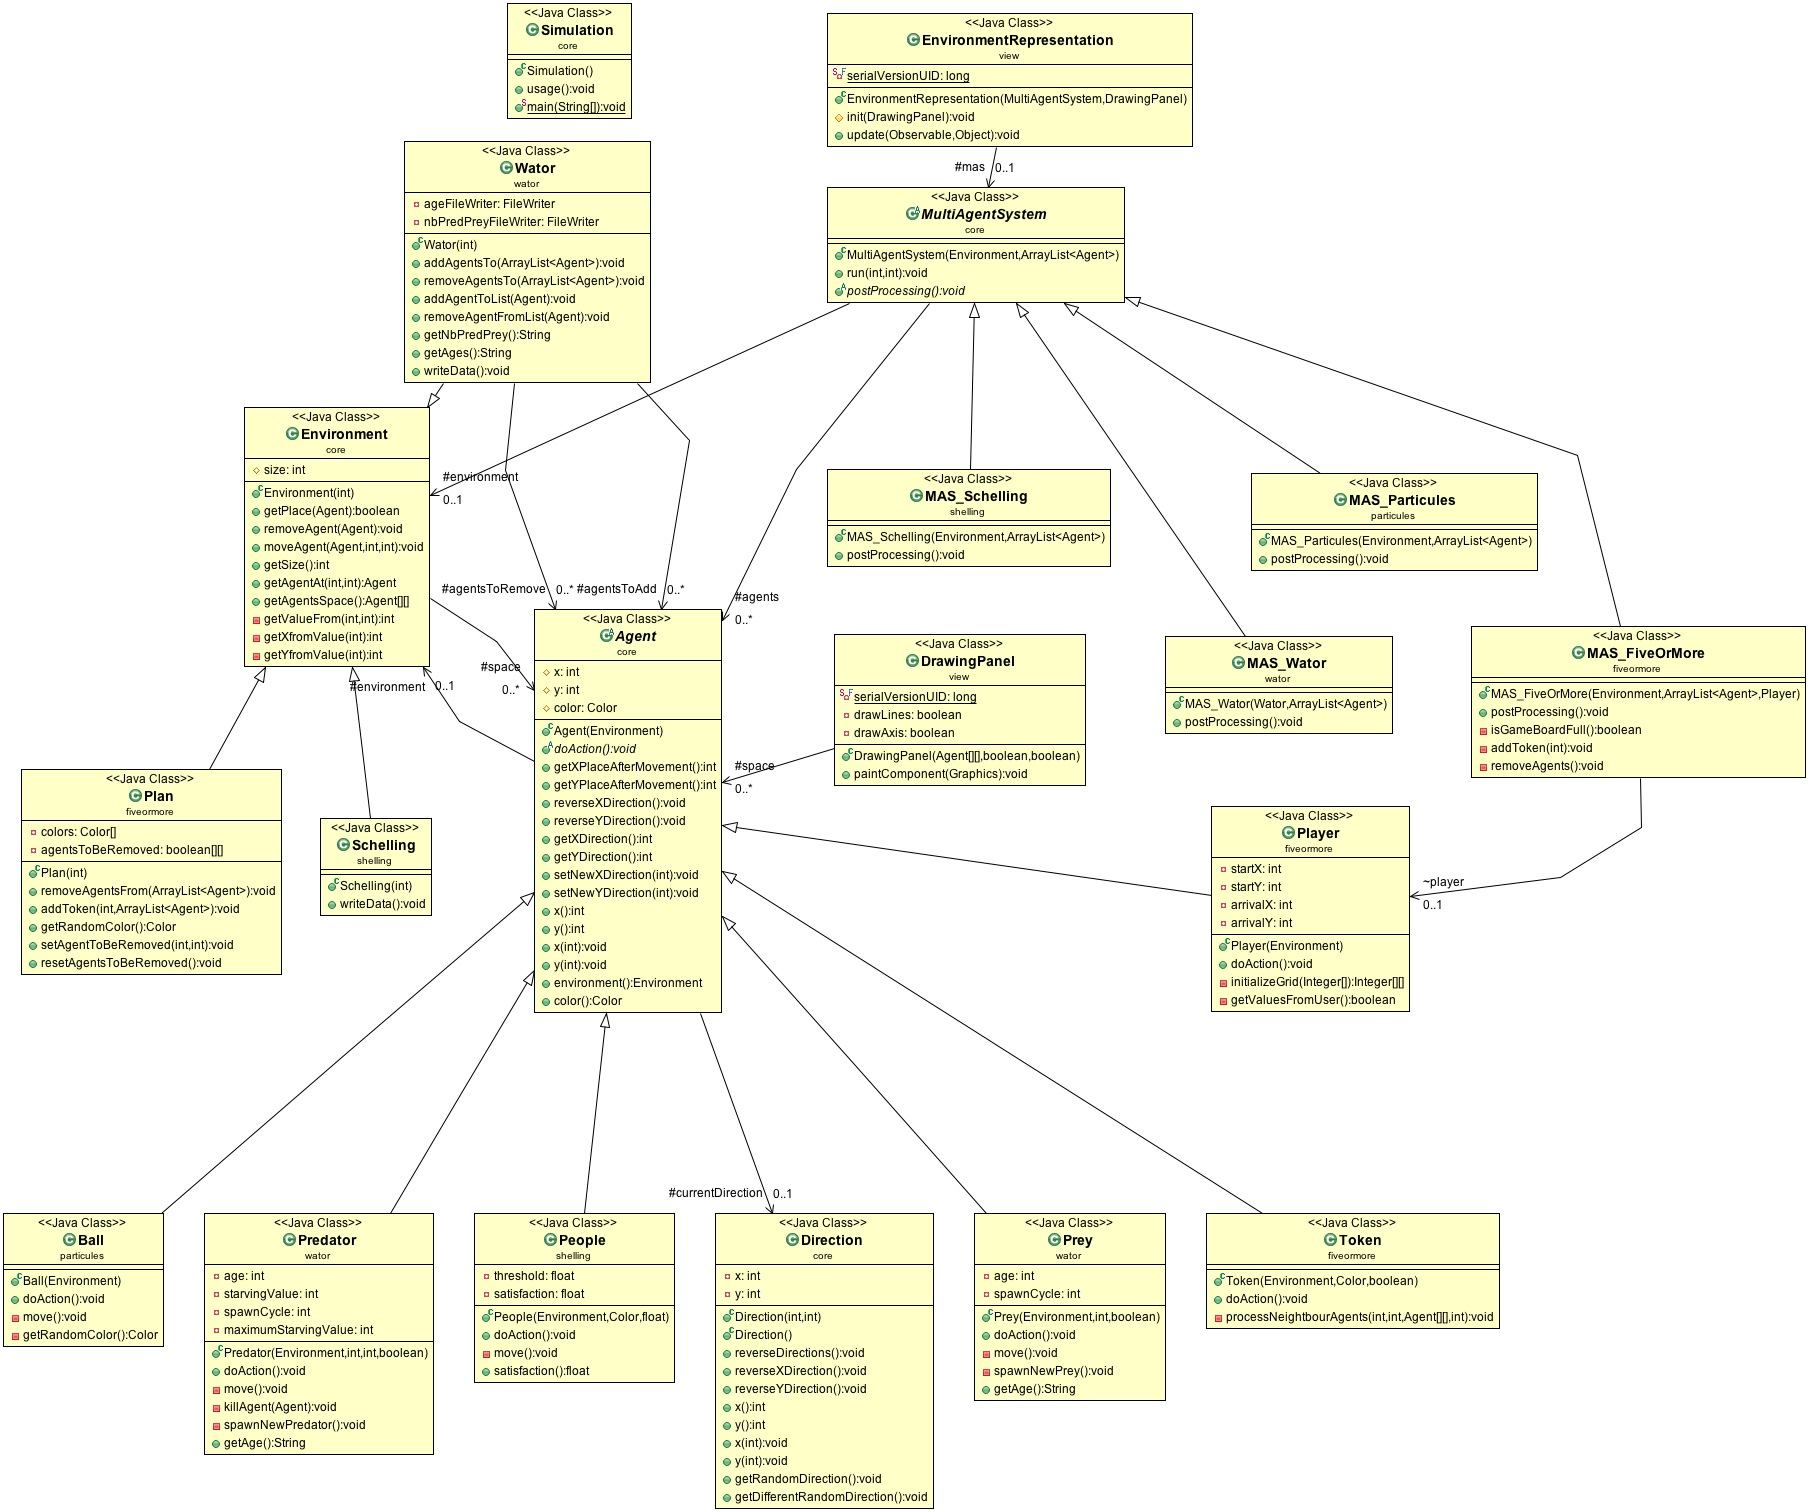
\includegraphics[width=17cm]{images/uml_tp3}
\end{center}
	\caption{L'UML du projet entier}
	\label{uml}
\end{figure}


\section{Compilation + fonctionnement}
 
\paragraph{Compilation} ~\\

Se mettre dans le dossier contenant le dossier src

\begin{Verbatim}[commandchars=\\\{\}]
mkdir bin
javac -sourcepath src -d bin src/core/Simulation.java
\end{Verbatim}

Ne pas bouger du dossier 

\paragraph{Execution} ~\\
Si on rentre un nombre de tour = -1 alors c'est infini \\

Pour la Simulation des Billes : \\ 
\verb&java -cp bin core.Simulation -b <taille> <nb agent> <nb tour> <delai entre chaque tour>& \\

Pour la Simulation du mod\`ele de Shelling : \\ 
\verb&java -cp bin core.Simulation -s <taille> <nb habitant> <seuil tolerance> <nb tour> <delai>& \\
Avec le seuil de tol\'erance compris entre 0 et 1. \\

Pour la Simulation du mod\`ele de Proies - P\'edateur : \\ 
\verb&java -cp bin core.Simulation -w <taille> <nb proies> <nb pred> <tps reprod proies>&

\verb&<tps reprod pred> <tps faim> <delai>& \\
 
 Pour la Simulation du jeu Cinq ou plus: \\ 
\verb&java -cp bin core.Simulation -f& \\

\paragraph{Exemples} ~\\

Billes : \\
~
\verb&java -cp bin core.Simulation -b 100 50 -1 5& \\
\verb&java -cp bin core.Simulation -b 10 5 100 5& \\
\verb&java -cp bin core.Simulation -b 50 40 -1 5& \\

Shelling : \\
~
\verb&java -cp bin core.Simulation -s 100 9750 0.3 -1 1& \\
\verb&java -cp bin core.Simulation -s 100 9750 0.6 -1 1 & \\
\verb&java -cp bin core.Simulation -s 50 2000 0.7 -1 100 & \\

Proies-Pr\'edateurs : \\
~
\verb&java -cp bin core.Simulation -w 50 1040 326 4 10 6 -1 50& \\
\verb&java -cp bin core.Simulation -w 10 10 5 4 10 6 -1 50& \\
\verb&java -cp bin core.Simulation -w 35 100 30 4 10 6 -1 50& \\

Cinq ou plus : \\
~
\verb&java -cp bin core.Simulation -f&

\section{Probl\`eme}

Nous n'avons plus de probl\`emes concernant proie - pr\'edateur et Schelling. Les valeurs sont bonnes (\emph{cf.} figure avec le rapport)

\end{document}